In this chapter we are going to study in deep the basic concepts about learning rule. With  \textit{learning rule} it means all the rules and algorithms used to modify the weight and the bias of the network in order to improve the results.
There are three main approaches:
\begin{itemize}
\item \textit{Supervised learning}. In this case the net is trained by using a set of examples composed by $(p_0, t_0)$ where $p_0$ is the input for the network and $t_0$ the corresponding correct result (target). The result produced is compared to the target. The learning rules are used to modify weights to make model produce the right result. 
\item \textit{Reinforcement Learning}. The algorithm produce a score or a grade according to the network performance and the learning rule seek to adjust weights in order to get higher scores. The network continues to learn also during its application.  
\item \textit{Unsupervised Learning}. The data does not have the target but they are somehow clustered. The cluster becomes the target to predict like the one in the supervised learning.
\end{itemize}

Probably, we will speak about all this approaches later.

\section{Learning rules for Perceptron Architecture}

\subsection{Perceptron Network again}
\begin{figure}
    \centering
    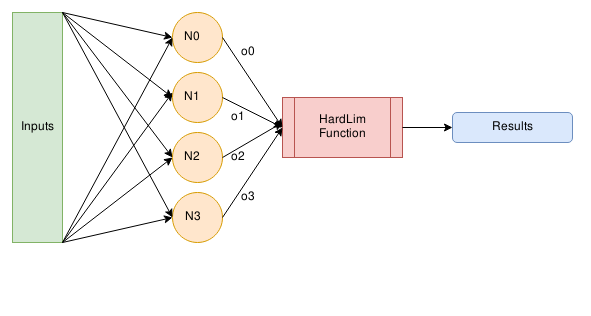
\includegraphics[scale=0.65]{img/PerceptronNetwork.png}
    \caption{Overview of a Perceptron Network}
    \label{img:perceptron_network}
\end{figure}
The perceptron network has a single layer of $S$ neurons and it use as activation function the \textbf{Hardlim} (it produce 0 or 1 according to the output of the neuron).
The weights of the network are:
\begin{equation}
\textbf{W} = \begin{bmatrix}
\textbf{w}_0 \\ \textbf{w}_1 \\ \vdots \\ \textbf{w}_s 
\end{bmatrix}
\end{equation}

So each neuron has a list of $w_{n0}, ... , w_{nm}$ weights where $n$ it the neuron and $m$ is the number of weight and it is the same for the number of inputs.

Each neuron produce a result $o_n$ and the list with all results from all neurons is given to the activation function.

\section*{the decision boundary}
Let's use a Perceptron Network with one neuron and 2 inputs. The result is obtained by this formula:
\begin{equation}
o = hardlim((w_0 * p_0 + w_1 * p_1) + b)
\end{equation}
The decision boundary of the network is determined by the sub set of inputs that make the neurons produce zeros.
\newline
\textbf{Example:}
Let's have $w_0 = 1$, $w_1= 1$ and $b = -1$. So the decision boundary will be:
\begin{equation}
(w_0 * p_0 + w_1 * p_1) + b = p_0 + p_1 - 1 = 0 \Rightarrow p_0 + p_1 = 1
\end{equation} 

The decision boundary define a line in the input space. On one side of that line, the network output will be 0, on the other side will be one.
\begin{figure}
    \centering
    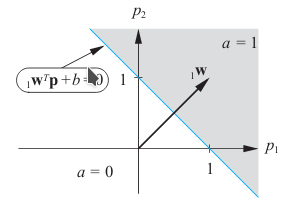
\includegraphics[scale=0.5]{img/decision_boundary_for_perceptron.png}
    \caption{Graphic representation of the decision boundary}
    \label{img:perceptron_network}
\end{figure}
Modifying the weights and the bias of the network this line is moved up and down changing also its orientation.

\subsection{Decision Boundary for Multiple Neurons}
Network with $S$ neurons has $S$ lines, one for each of them. So each neuron can classify each input in just two categories. A network with one neuron has one decision boundary so it can produce just 2 category, while a network with S neurons can produce $2^s$ different output vectors so it can be used to classify an input to these categories.

\section{Learning rules for Perceptron Network}
There is a precise algorithm that tells us how to update the weights and it guarantees the best solution is found.
The idea behind is if the model predict the wrong result weight must be modified to let the model classify that input. For this case let's define $e = t - a$ where $t$ is the target and $a$ is the output of the model. Each weight is updated according to this formula:
\begin{equation}
\textbf{w}^{new} = \textbf{w}^{old} + e\textbf{p}
\end{equation}
We can do the same for bias: Bias are just single weight for an input that is always one.
\begin{equation}
b^{new} = b^{old} + e
\end{equation}

So, the perceptron rule can be written for the matrix of weight in case the network has more than one neuron.

\begin{equation}
\textbf{W}^{new} = \textbf{W}^{old} + \textbf{e}\textbf{p}
\end{equation}
\begin{equation}
\textbf{b}^{new} = \textbf{b}^{old} + \textbf{e}
\end{equation}

\textit{That is all by now, but there is a proof of convergence that demonstrates this algorithm always find the best solution}.

\subsection{Example}
Let's have a singular-neuron perceptron network for 3-input vectors: $i_0 = [1,-1,0]$, $i_1 = [1,1,-1]$, $i_2 = [1,0,0]$. For all of them we have the corresponding targets $t_0 = 1,  t_1 = 0,  t_2 = 1$. Let's initialize our net with random values: $w = [0, 0.5, -0.2], b = 0.3$.
\newline
First, it can be useful find out the decision boundary:
\begin{equation}
(0*i_{n0} + 0.5 * i_{n1} - 0.2 * i_{n2}) + 0.3) = 0 \Rightarrow \frac{i_{n1}}{2} - \frac{i_{n2}}{5} = 0.3
\end{equation}

Now we can proceed giving the first input to the network and see what happend:
\begin{equation}
hardlim((0*1 + 0.5 * -1 - 0.2 * 0) + 0.3) = hardlim(0 - 0,5 + 0 + 0.3) = hardlim(-0,2) = 0 
\end{equation}
So $e = t - a = 1 - 0 = 1$. Let's apply the updating formula :
\begin{equation}
\textbf{w}^{new} = \textbf{w}^{old} + e\textbf{p} = [0, 0.5, -0.2] + (1)[1, -1, 0] = [1, -0.5, -0.2]
\end{equation}
\begin{equation}
b^{new} = b^{old} + e = 0.3 + (1)= 1.3
\end{equation}

Let's do it again but with the second input. (I gonna skip some calculus)
\begin{equation}
hardlim((1*1 + -0.5 * 1 - 0.2 * -1) + 1.3) = hardlim(2) = 1 
\end{equation}
Again the model mistakes. $e = t - a = -1$. So let's repeat the update phase:
\begin{equation}
\textbf{w}^{new} = \textbf{w}^{old} + e\textbf{p} = [1,-0.5,-0.2] + (-1)[1, 1, -1] = [0, -1.5, 0.8]
\end{equation}
\begin{equation}
b^{new} = b^{old} + e = 1.3 + (-1)= 0.3
\end{equation}

Let's do it again but with the third input. (I gonna skip some calculus)
\begin{equation}
hardlim((0*1 - 1.5 * 0 + 0.8 * 0) + 0.3) = hardlim(0.3) = 1 
\end{equation}
This time the prediction is good and $e = 0$

Let's test the new weights with the first input:
\begin{equation}
hardlim((0*1 - 1.5 * -1 + 0.8 * 0) + 0.3) = hardlim(1.8) = 1 
\end{equation}
Good, it is correct. And at last, let's check for second input:
\begin{equation}
hardlim((0*1 - 1.5 * 1 + 0.8 * -1) + 0.3) = hardlim(-2) = 0 
\end{equation}
That is cool! Now model can predict the right result for all of them!



\section{Perceptron Network Limitation}

This network can find the best solution of classification problem in a finite number of steps, however it can cut the input space using lines (hyperplane). It can't model create decision boundary not-linear, so if data are a long some curve they can't be classified. For example this network can learn to produce AND but it can't reproduce XOR. Try to think why by yourself.


